\documentclass[12pt]{article}

\usepackage[portuguese]{babel}
\usepackage{graphicx}
\usepackage[section]{placeins}
\usepackage{float}
\usepackage{url}

\graphicspath{ {figures} }

\author{João Vitor Maia Neves Cordeiro}
\title{Segundo trabalho prático: Wireshark e SNMP}
\date{\today}

\begin{document}

\maketitle

\section{Texto de requisitos}

Jogo de Quiz com perguntas e respostas, este é o trabalho que usaremos como alvo para modelar e desenvolver nosso banco de dados. Como o nome diz, consiste em um jogo onde serão dadas várias perguntas à um ou mais usuários e registrado a pontuação do usuário no jogo atual. Existem várias categorias de jogos e várias categorias de perguntas. As perguntas também serão registradas no banco, assim como suas alternativas corretas e incorretas. Também será possível que dois usuários se desafiem em um jogo.

Cada usuário poderá então participar tanto de jogos singleplayer quanto multiplayer desafiando outros jogadores, e para que isso seja possível o banco guardará o nome e e-mail deste jogador, registrando o mesmo com um id.

Por mais que seja possível desafiar outros jogadores, cada jogo é individual, tendo então apenas um usuário e um placar correspondendo aos pontos marcados pelo jogador.

Já o desafio é então a materialização de dois jogos, um sobre um jogador Y e outro sobre um jogador X, guardando tanto as informações sobre os jogadores quanto sobre os jogos para que possa mais tarde executar operações sobre os dados armazenados.

Também teremos as categorias do jogo, informando quais categorias de pergunta podem ser enviadas para o usuário de um devido jogo.

A categoria por sua vez será constituída de um título e um id para falicitar sua procura sobre as perguntas armazenadas.

E finalmente chegamos então nas perguntas, estas armazenarão tanto a pergunta em si quanto a categoria a qual elas pertencem.

Não menos importante que as perguntas, teremos as opções. Uma opção é composta por um boolean para dizer se ela é a resposta verdadeira ou a resposta falsa, além de ter a referência para a questão que ela responde e a resposta em si.

\section{Modelo conceitual}

\begin{figure}[H]
    \centering
    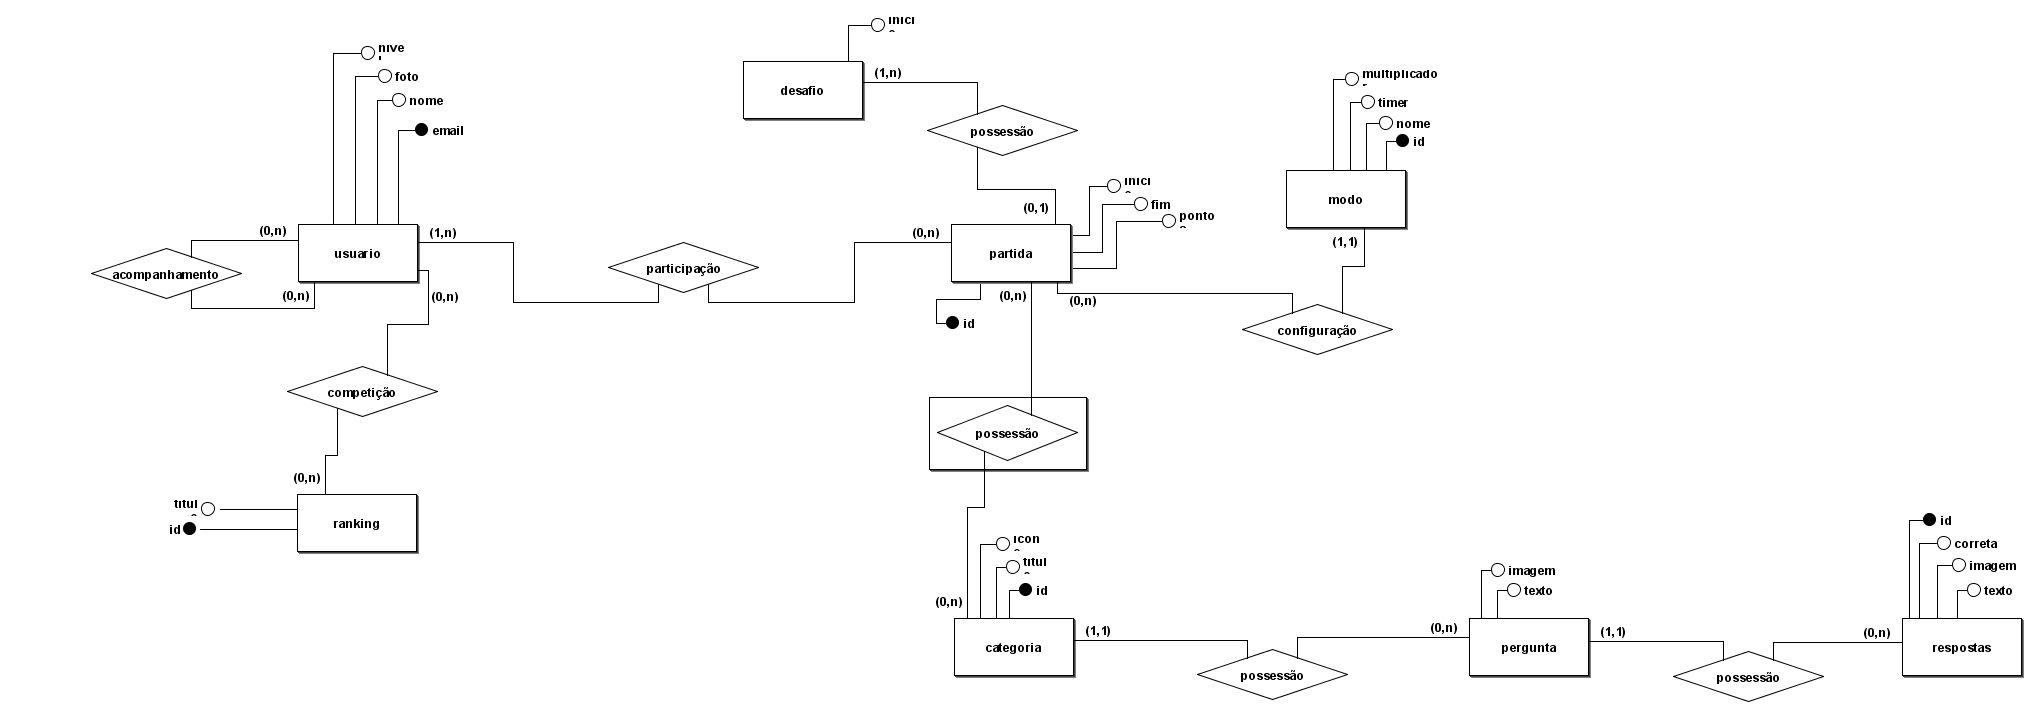
\includegraphics[width=\linewidth]{conceitual.png}
    \caption{Modelo conceitual.}
\end{figure}

\section{Modelo lógico}

\begin{figure}[H]
    \centering
    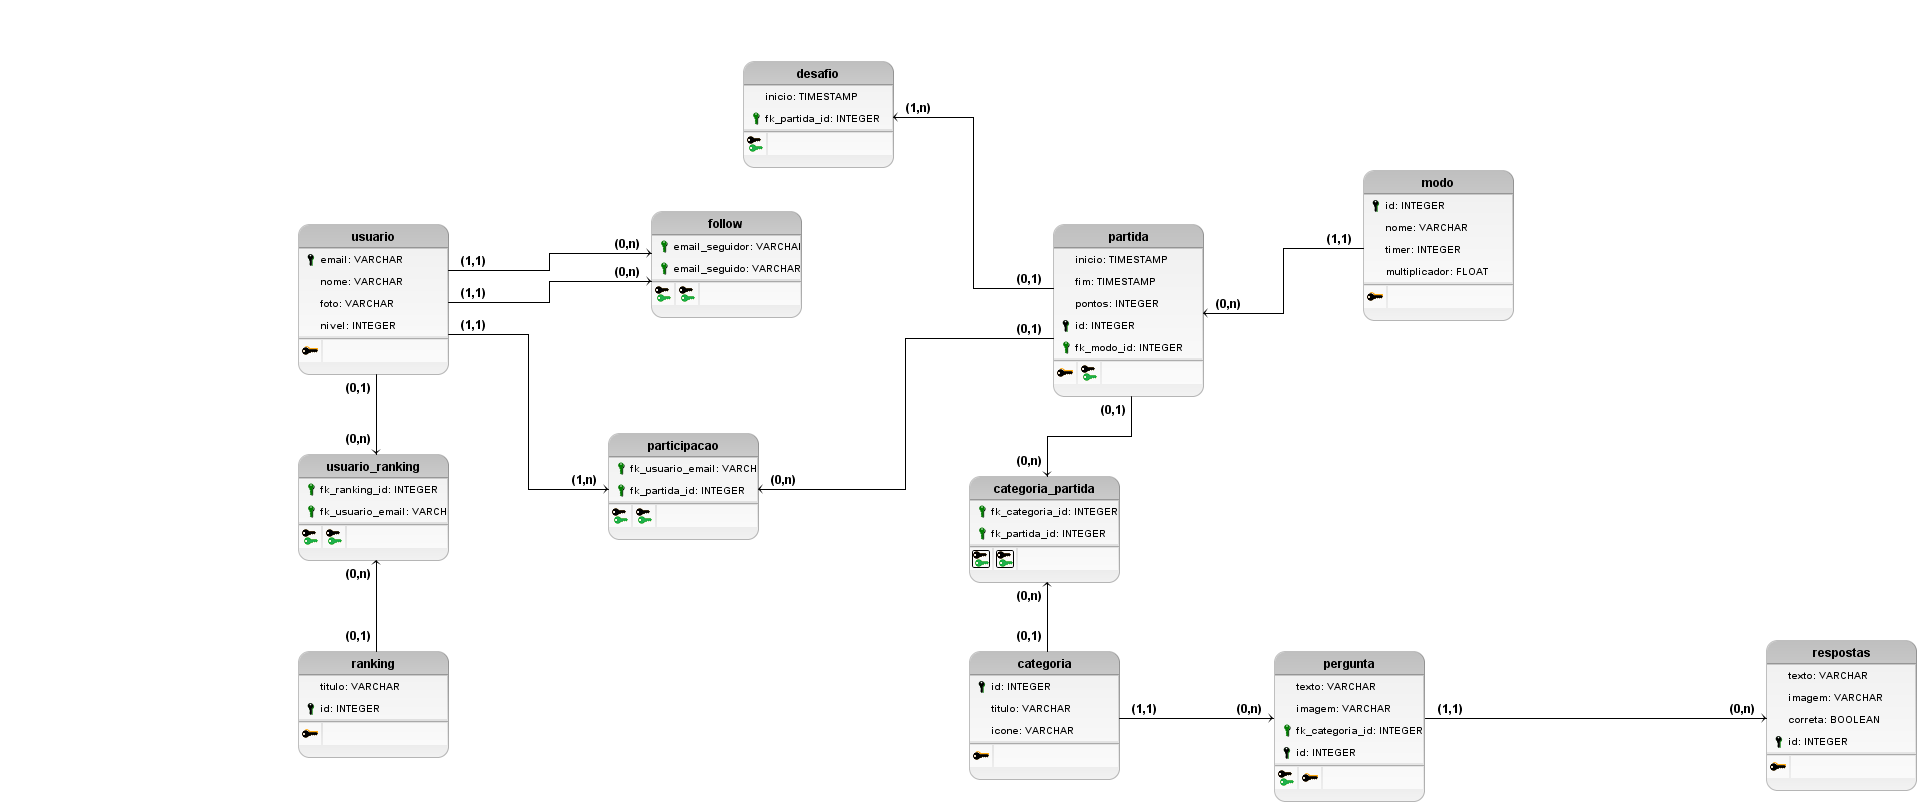
\includegraphics[width=\linewidth]{logico.png}
    \caption{Modelo lógico.}
\end{figure}

\section{Modelo físico}

\begin{lstlisting}[language=SQL]
CREATE TABLE usuario (
    email VARCHAR PRIMARY KEY,
    nome VARCHAR,
    foto TEXT,
    nivel INTEGER
);

CREATE TABLE modo (
    id INTEGER PRIMARY KEY,
    nome VARCHAR,
    timer INTEGER,
    multiplicador FLOAT
);

CREATE TABLE categoria (
    id INTEGER PRIMARY KEY,
    titulo VARCHAR,
    icone VARCHAR
);

CREATE TABLE partida (
    inicio TIMESTAMP,
    fim TIMESTAMP,
    pontos INTEGER,
    id INTEGER PRIMARY KEY,
    fk_modo_id INTEGER,
    FOREIGN KEY (fk_modo_id) REFERENCES modo(id)
);

CREATE TABLE pergunta (
    id INTEGER PRIMARY KEY
    texto TEXT,
    imagem TEXT,
    fk_categoria_id INTEGER,
    FOREIGN KEY (fk_categoria_id) REFERENCES categoria(id)
);

CREATE TABLE respostas (
    id INTEGER PRIMARY KEY,
    texto TEXT,
    imagem TEXT,
    correta BOOLEAN
);

CREATE TABLE categoria_partida (
    fk_categoria_id INTEGER,
    fk_partida_id INTEGER,
    FOREIGN KEY (fk_categoria_id) REFERENCES categoria(id),
    FOREIGN KEY (fk_partida_id) REFERENCES partida(id)
);

CREATE TABLE desafio (
    inicio TIMESTAMP,
    fk_partida_id INTEGER,
    FOREIGN KEY (fk_partida_id) REFERENCES partida(id)
);

CREATE TABLE ranking (
    id INTEGER PRIMARY KEY,
    titulo VARCHAR
);

CREATE TABLE follow (
    email_seguidor VARCHAR,
    email_seguido VARCHAR,
    FOREIGN KEY (email_seguidor) REFERENCES usuario(email),
    FOREIGN KEY (email_seguido) REFERENCES usuario(email)
);

CREATE TABLE participacao (
    fk_usuario_email VARCHAR,
    fk_partida_id INTEGER,
    FOREIGN KEY (fk_usuario_email) REFERENCES usuario(email),
    FOREIGN KEY (fk_partida_id) REFERENCES partida(id)
);

CREATE TABLE usuario_ranking (
    fk_ranking_id INTEGER,
    fk_usuario_email VARCHAR,
    FOREIGN KEY (fk_ranking_id) REFERENCES ranking(id),
    FOREIGN KEY (fk_usuario_email) REFERENCES usuario(email)
);
\end{lstlisting}

\nocite{*}
\medskip

\bibliographystyle{abbrv}
\bibliography{biblio}

\end{document}